% F049: native TikZ/PGFPlots, computed from the stated mathematical model.
\begin{center}
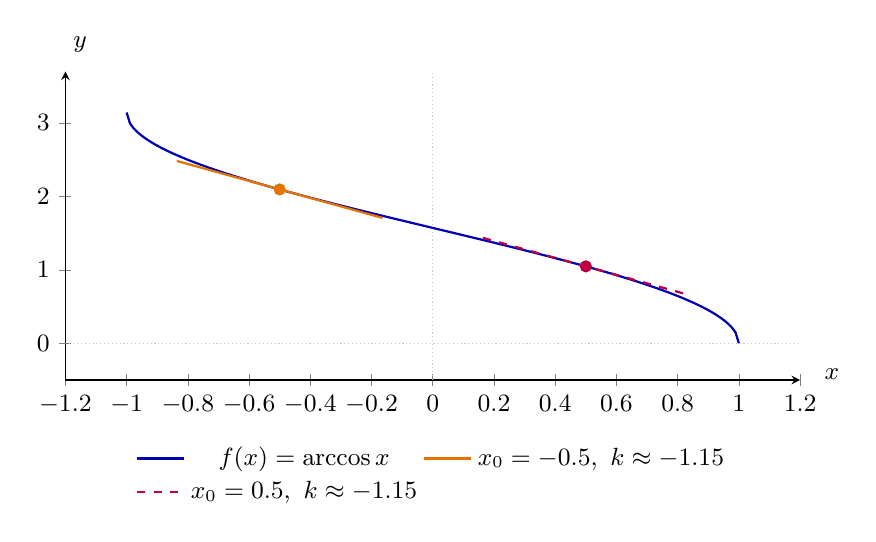
\begin{tikzpicture}[font=\small,>=stealth]
\begin{axis}[width=.90\linewidth,height=5.5cm,xmin=-1.2,xmax=1.2,ymin=-0.5,ymax=3.7,
axis lines=left,xlabel={$x$},ylabel={$y$},font=\small,
xlabel style={at={(axis description cs:1.02,.02)},anchor=west},
ylabel style={rotate=-90,at={(axis description cs:.02,1.03)},anchor=south},
legend style={at={(axis description cs:.5,-.18)},anchor=north,draw=none,fill=none,font=\small,legend columns=2},
unbounded coords=jump,clip=true,]
\addplot[gray!45,thin,densely dotted,forget plot] coordinates {(-1.2,0) (1.2,0)};
\addplot[gray!45,thin,densely dotted,forget plot] coordinates {(0,-0.5) (0,3.7)};
\addplot[blue!70!black,thick] coordinates {(-1,3.1415927) (-0.98888889,2.9923831) (-0.97777778,2.9303818) (-0.96666667,2.8826711) (-0.95555556,2.8423348) (-0.94444444,2.8066965) (-0.93333333,2.7743846) (-0.92222222,2.7445852) (-0.91111111,2.7167682) (-0.9,2.6905658) (-0.88888889,2.6657104) (-0.87777778,2.642) (-0.86666667,2.6192778) (-0.85555556,2.5974193) (-0.84444444,2.5763235) (-0.83333333,2.5559071) (-0.82222222,2.5361008) (-0.81111111,2.5168456) (-0.8,2.4980915) (-0.78888889,2.4797952) (-0.77777778,2.4619188) (-0.76666667,2.4444295) (-0.75555556,2.4272981) (-0.74444444,2.4104987) (-0.73333333,2.3940083) (-0.72222222,2.3778062) (-0.71111111,2.3618736) (-0.7,2.3461938) (-0.68888889,2.3307514) (-0.67777778,2.3155324) (-0.66666667,2.300524) (-0.65555556,2.2857144) (-0.64444444,2.2710928) (-0.63333333,2.2566493) (-0.62222222,2.2423745) (-0.61111111,2.2282599) (-0.6,2.2142974) (-0.58888889,2.2004797) (-0.57777778,2.1867997) (-0.56666667,2.173251) (-0.55555556,2.1598273) (-0.54444444,2.146523) (-0.53333333,2.1333326) (-0.52222222,2.120251) (-0.51111111,2.1072733) (-0.5,2.0943951) (-0.48888889,2.0816119) (-0.47777778,2.0689197) (-0.46666667,2.0563144) (-0.45555556,2.0437925) (-0.44444444,2.0313503) (-0.43333333,2.0189845) (-0.42222222,2.0066917) (-0.41111111,1.9944689) (-0.4,1.9823132) (-0.38888889,1.9702216) (-0.37777778,1.9581914) (-0.36666667,1.9462199) (-0.35555556,1.9343047) (-0.34444444,1.9224433) (-0.33333333,1.9106332) (-0.32222222,1.8988723) (-0.31111111,1.8871583) (-0.3,1.875489) (-0.28888889,1.8638624) (-0.27777778,1.8522764) (-0.26666667,1.8407291) (-0.25555556,1.8292186) (-0.24444444,1.817743) (-0.23333333,1.8063006) (-0.22222222,1.7948894) (-0.21111111,1.7835079) (-0.2,1.7721542) (-0.18888889,1.7608269) (-0.17777778,1.7495241) (-0.16666667,1.7382444) (-0.15555556,1.7269862) (-0.14444444,1.7157478) (-0.13333333,1.7045279) (-0.12222222,1.6933249) (-0.11111111,1.6821373) (-0.1,1.6709637) (-0.088888889,1.6598027) (-0.077777778,1.6486527) (-0.066666667,1.6375125) (-0.055555556,1.6263805) (-0.044444444,1.6152554) (-0.033333333,1.6041358) (-0.022222222,1.5930204) (-0.011111111,1.5819077) (0,1.5707963) (0.011111111,1.559685) (0.022222222,1.5485723) (0.033333333,1.5374568) (0.044444444,1.5263372) (0.055555556,1.5152122) (0.066666667,1.5040802) (0.077777778,1.4929399) (0.088888889,1.48179) (0.1,1.4706289) (0.11111111,1.4594553) (0.12222222,1.4482677) (0.13333333,1.4370647) (0.14444444,1.4258448) (0.15555556,1.4146065) (0.16666667,1.4033482) (0.17777778,1.3920685) (0.18888889,1.3807658) (0.2,1.3694384) (0.21111111,1.3580848) (0.22222222,1.3467032) (0.23333333,1.3352921) (0.24444444,1.3238496) (0.25555556,1.312374) (0.26666667,1.3008635) (0.27777778,1.2893163) (0.28888889,1.2777303) (0.3,1.2661037) (0.31111111,1.2544344) (0.32222222,1.2427204) (0.33333333,1.2309594) (0.34444444,1.2191494) (0.35555556,1.2072879) (0.36666667,1.1953727) (0.37777778,1.1834013) (0.38888889,1.1713711) (0.4,1.1592795) (0.41111111,1.1471237) (0.42222222,1.134901) (0.43333333,1.1226082) (0.44444444,1.1102423) (0.45555556,1.0978001) (0.46666667,1.0852782) (0.47777778,1.072673) (0.48888889,1.0599807) (0.5,1.0471976) (0.51111111,1.0343193) (0.52222222,1.0213417) (0.53333333,1.0082601) (0.54444444,0.99506968) (0.55555556,0.98176536) (0.56666667,0.96834169) (0.57777778,0.95479293) (0.58888889,0.94111295) (0.6,0.92729522) (0.61111111,0.91333277) (0.62222222,0.89921815) (0.63333333,0.88494336) (0.64444444,0.87049981) (0.65555556,0.85587825) (0.66666667,0.84106867) (0.67777778,0.82606025) (0.68888889,0.81084124) (0.7,0.79539883) (0.71111111,0.77971903) (0.72222222,0.7637865) (0.73333333,0.74758435) (0.74444444,0.73109394) (0.75555556,0.71429455) (0.76666667,0.69716313) (0.77777778,0.67967382) (0.78888889,0.66179748) (0.8,0.64350111) (0.81111111,0.62474702) (0.82222222,0.6054919) (0.83333333,0.58568554) (0.84444444,0.56526918) (0.85555556,0.54417334) (0.86666667,0.52231482) (0.87777778,0.49959266) (0.88888889,0.47588225) (0.9,0.45102681) (0.91111111,0.42482443) (0.92222222,0.39700745) (0.93333333,0.36720802) (0.94444444,0.33489616) (0.95555556,0.29925782) (0.96666667,0.25892154) (0.97777778,0.21121088) (0.98888889,0.14920957) (1,0)};
\addlegendentry{$f(x)=\arccos x$}
\addplot[orange!90!black,thick] coordinates {(-0.836,2.4823745) (-0.164,1.7064157)};
\addlegendentry{$x_0=-0.5,\ k\approx-1.15$}
\addplot[only marks,mark=*,orange!90!black,forget plot] coordinates {(-0.5,2.0943951)};
\addplot[purple,thick,dashed] coordinates {(0.164,1.4351769) (0.836,0.65921817)};
\addlegendentry{$x_0=0.5,\ k\approx-1.15$}
\addplot[only marks,mark=*,purple,forget plot] coordinates {(0.5,1.0471976)};

\end{axis}
\end{tikzpicture}
\par\smallskip{\small 拓展；$|x|<1$，导数为负，图像递减。}
\end{center}
